% exercise sheet with header on every page for math or close subjects
\documentclass[12pt]{article}
\usepackage[utf8]{inputenc} 
\usepackage{latexsym} 
\usepackage{multicol}
\usepackage{fancyhdr}
\usepackage{amsfonts} 
\usepackage{amsmath}
\usepackage{amssymb}
\usepackage{enumerate}
\usepackage{listings}
\usepackage{graphicx}
\usepackage{hyperref}

% Shortcuts for bb, frak and cal letters
\newcommand{\E}{\mathbb{E}}
\newcommand{\V}{\mathbb{V}}
\renewcommand{\P}{\mathbb{P}}
\newcommand{\N}{\mathbb{N}}
\newcommand{\R}{\mathbb{R}}
\newcommand{\C}{\mathbb{C}}
\newcommand{\Z}{\mathbb{Z}}
\newcommand{\Pfrak}{\mathfrak{P}}
\newcommand{\Pfrac}{\mathfrak{P}}
\newcommand{\Bfrac}{\mathfrak{P}}
\newcommand{\Bfrak}{\mathfrak{B}}
\newcommand{\Fcal}{\mathcal{F}}
\newcommand{\Ycal}{\mathcal{Y}}
\newcommand{\Bcal}{\mathcal{B}}
\newcommand{\Acal}{\mathcal{A}}

% formating
\topmargin -1.5cm 
\textheight 24cm
\textwidth 16.0 cm 
\oddsidemargin -0.1cm

% Fancy Header on every Page
\pagestyle{fancy}
\lhead{\textbf{Pattern and Speech Recognition}}
\rhead{Daniel Schäfer (2549458)\\ Christian Bohnenberger (2548364) \\ Dominik Weber (2548553)}
\renewcommand{\headrulewidth}{1.2pt}

\setlength{\headheight}{45pt} 

\begin{document}
\pagenumbering{gobble}

% TODO set the number of the exercise sheet here!
\setcounter{section}{8}
\setcounter{subsection}{0}

\subsection{ }

\begin{enumerate}[a)]
\item
\begin{itemize}
	\item $s_1[0]= 0.5 * 3 = 1.5 $
	\item $s_1[1]= 0.5 * 3 + 0.5 * 1 = 2 $
	\item $s_1[2]= 0.5 * 1 + 0.5 * 8 = 4.5 $	
	\item $s_1[3]= 0.5 * 8 + 0.5 * 6 = 7 $
	\item $s_1[4]= 0.5 * 6 + 0.5 * 3 = 4.5 $	
	\item $s_1[5]= 0.5 * 3 + 0.5 * 9 = 6 $
	\item $s_1[6]= 0.5 * 9 + 0.5 * 5 = 7 $
	\item $s_1[7]= 0.5 * 5 + 0.5 * 1 = 3 $
	\item $s_1[8]= 0.5 * 1 = 0.5 $
\end{itemize}
$s_1$=\begin{tabular}{|c|c|c|c|c|c|c|c|c|}
\hline
1.5 & 2 & 4.5 & 7 & 4.5 & 6 & 7 & 3 & 0.5\\ \hline
\end{tabular}
\item
computation as in a.) \\
$s_2=$\begin{tabular}{|c|c|c|c|c|c|c|c|c|c|}
\hline
0.75 & 1.75 & 3.25 & 5.75 & 5.75 & 5.25 & 6.5 & 5 & 1.75 & 0.25\\ \hline
\end{tabular}

\item
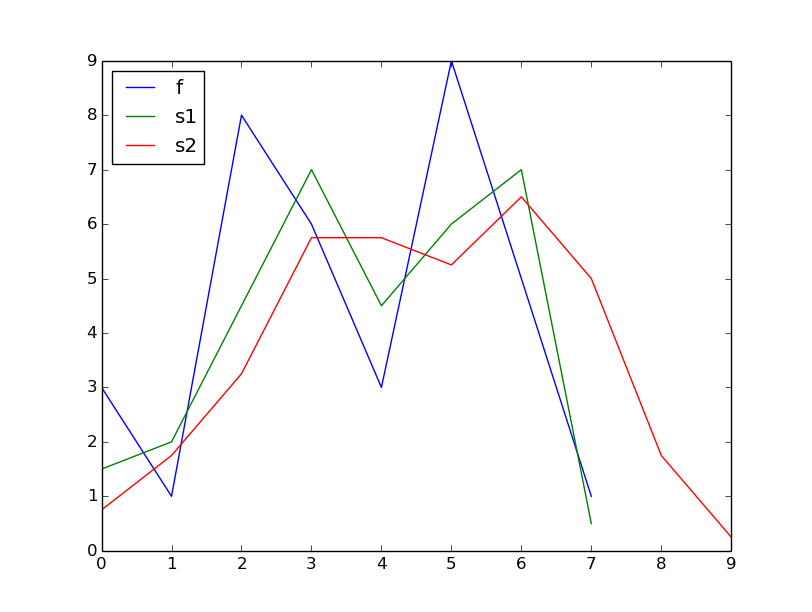
\includegraphics[scale=0.4]{plot81c.png}
The outcome increases the size by 1 every times we use convolution. Furthermore, we can see the values on the edges are very small. And they will be be smaller every times we apply convolution. The big gap between the values in the middle which is given in $f$ is decreased every times convolution is applied. If we apply convolution $n$-times and $n \rightarrow \infty$ we get the values in the middle at about the same value, whereas the values next on the edges are close to 0. In the end the the amplitude will be flattened.

\item
\begin{itemize}
	\item $k'[0]=0.25$
	\item $k'[0]=0.5$
	\item $k'[0]=0.25$\\
	$\Rightarrow k'= $\begin{tabular}{|c|c|c|}
	\hline 0.25 & 0.5 & 0.25 \\ \hline
	\end{tabular}
	\item $s_3[0]= 0.25*3= 0.75$
	\item $s_3[1]= 0.25*1+0.5*3=1.75$
	\item $s_3[2]= 0.25*8+0.5*1+0.25*3=3.25$
	\item \dots \\
	$\Rightarrow s_3=$
	\begin{tabular}{|c|c|c|c|c|c|c|c|c|c|}
		\hline
		0.75 & 1.75 & 3.25 & 5.75 & 5.75 & 5.25 & 6.5 & 5 & 1.75 & 0.25\\ \hline
	\end{tabular}
\end{itemize}

\item 
\begin{itemize}
	\item $s_2$ and $s_3$ are equal that means $(f*k)*k=f*(k*k)$
	\item associativity seems to be fullfilled by convolution
	\item Proof:\\
	We want to show: $(f*g)*h=f*(g*h)$:\\
	$$((f*g)*h)(t) =^{Definition} \int (f*g)(a)*h(t-a) da $$
	$$ =^{Definition} \int (\int f(b)*g(a-b) db)*h(t-a) da $$
	$$=^{Definition}\int \int f(b)*g(a-b)*h(t-a) db~ da $$
	$$=^{Fubini} \int \int f(b)*g(a-b)*h(t-a) da~ db$$
	$$=^{Definition} \int f(b) (\int g(a-b)*h(t-a) da) db$$
	$$=^{Definition} \int f(b)(\int g(a) * h((t-b)-a) da) db $$
	$$=^{Definition} \int f(b) (g*h)(t-b) db$$
	$$=^{Definition} (f*(g*h))(t) $$
\end{itemize}
\end{enumerate}


\newpage
\subsection{ }
\begin{enumerate}[a)]
    \item 
        The function \verb!conv(image, kernel)! in \verb!convolution.py! implements said convolution.

    \item
        Output see Figure \ref{fig:conv82b}\\
        This Kernel applies smoothing on the picture. It esentially averages the color of every pixel to the average gray-value of the pixel and all its ``neighbour-pixels''. This obviously makes edges appear much more smooth and also reduces noise in the picture.\\
        $\Rightarrow$ this effect is called box blur or normalized blur.

        \begin{figure}
          \centering
            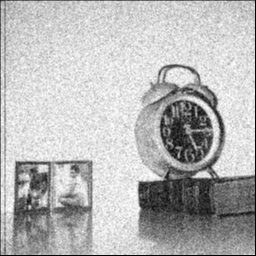
\includegraphics[scale = 1.00]{pictures/conv_b}
          \caption{convolution from exercise 8.2 b)}
          \label{fig:conv82b}
        \end{figure}

    \item
        Output see Figure \ref{fig:conv82c}\\
        This Kernel applies vertical edge detection! It can be used to detect vertical edges in all kind of scenarios. Bright points in the resulting picture are detected vertical edges in the original picture which occur on dark points which are surrounded by brighter pixels on the right and/or left. Very dark points in the resulting picture occur when a bright pixel in the original picture is surrounded by 2 much darker pixels on the right and/or left.\\

        \begin{figure}
          \centering
            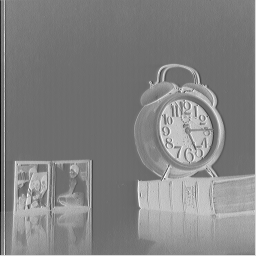
\includegraphics[scale = 1.00]{pictures/conv_c}
          \caption{convolution from exercise 8.2 c)}
          \label{fig:conv82c}
        \end{figure}

    \item
        because zero represents the darkest black possible it obviously creates very sharp edges for the outer most rows and columns in our padded picture, because the color difference between all pixels in these outer most columns and rows and their neighbours (pixels contained in the unpadded picture) can be very big. For our example picture a white instead of black padding would have been a lot better obviously. A better approach for the padded pixels would be if they contain the average color of their adjacent pixels. This would minimize this problem while still being very easy to compute.\\

\end{enumerate}



\subsection{ }
The execution of the CNN \verb!cnn.py! yields the following results:

\begin{center}
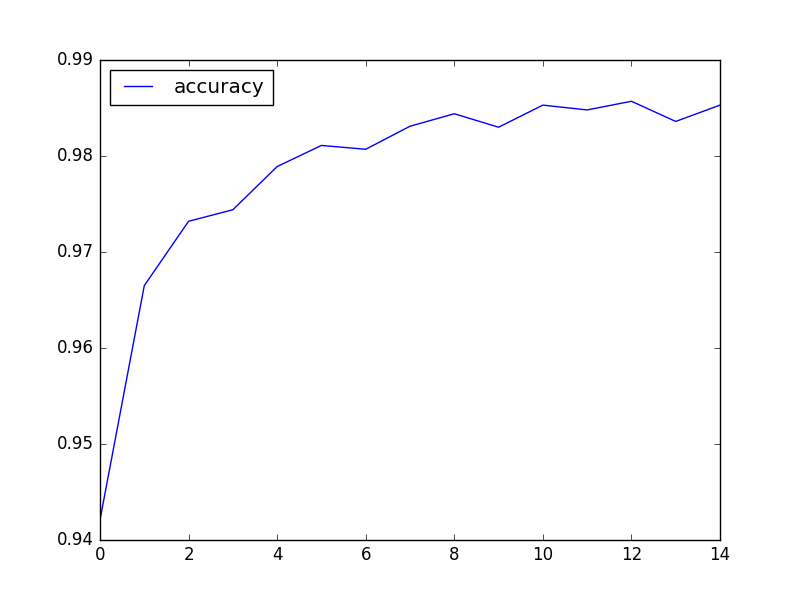
\includegraphics[scale = 0.60]{pictures/cnn_perf}
\end{center}

\newpage
\begin{verbatim}
Epoch: 0001 cost= 0.416582565
Accuracy on test-set: 0.9421
Epoch: 0002 cost= 0.151635871
Accuracy on test-set: 0.9665
Epoch: 0003 cost= 0.101485111
Accuracy on test-set: 0.9732
Epoch: 0004 cost= 0.076626663
Accuracy on test-set: 0.9744
Epoch: 0005 cost= 0.060655135
Accuracy on test-set: 0.9789
Epoch: 0006 cost= 0.049003780
Accuracy on test-set: 0.9811
Epoch: 0007 cost= 0.042118811
Accuracy on test-set: 0.9807
Epoch: 0008 cost= 0.036145066
Accuracy on test-set: 0.9831
Epoch: 0009 cost= 0.029712487
Accuracy on test-set: 0.9844
Epoch: 0010 cost= 0.025284777
Accuracy on test-set: 0.983
Epoch: 0011 cost= 0.020467684
Accuracy on test-set: 0.9853
Epoch: 0012 cost= 0.018045063
Accuracy on test-set: 0.9848
Epoch: 0013 cost= 0.016438036
Accuracy on test-set: 0.9857
Epoch: 0014 cost= 0.012611102
Accuracy on test-set: 0.9836
Epoch: 0015 cost= 0.012112769
Accuracy on test-set: 0.9853
Optimization Finished!
Accuracy on test-set: 0.9853
\end{verbatim}

After 15 epochs our CNN was able to achieve an Accuracy of 98,53\% on the test-set as you can see in the figure above.


\newpage
\subsection{ }
see code \verb!gabor_filter.py!

\end{document}
